\documentclass[11pt, a4paper]{article}

% Pakiety podstawowe i językowe
\usepackage[a4paper, top=2.5cm, bottom=2.5cm, left=2.5cm, right=2.5cm]{geometry}

% POPRAWKA BŁĘDU KOMPILACJI: Zmiana z XeTeX/LuaTeX na standardowy pdfTeX (używający T1 i UTF-8)
\usepackage[T1]{fontenc} 
\usepackage[utf8]{inputenc}
\usepackage[polish]{babel}

% Pakiety matematyczne i tabelaryczne
\usepackage{amsmath}
\usepackage{amssymb}
\usepackage{amsthm}
\usepackage{graphicx}
\usepackage{booktabs}
\usepackage{multirow} % Wymagany do grupowania wierszy w tabelach (jak w wynikach P2P)

% Formatowanie dokumentu
\title{Sprawozdanie z Laboratorium 3: Porównanie implementacji algorytmu Dijkstry}
\author{Kajetan Plewa}
\date{Grudzień 2025}

\begin{document}
	\maketitle
	\thispagestyle{empty}
	\clearpage
	
	% --- WSTĘP ---
	\section*{Wstęp}
	
	Celem niniejszego sprawozdania jest analiza porównawcza wydajności trzech wariantów algorytmu Dijkstry, służącego do wyznaczania najkrótszych ścieżek z pojedynczego źródła (SSSP) w grafach z nieujemnymi wagami krawędzi. Badania zostały przeprowadzone na grafach o różnej charakterystyce, w tym na danych syntetycznych oraz rzeczywistych sieciach drogowych.
	
	W ramach realizacji zadania zaimplementowano i przetestowano następujące warianty:
	\begin{enumerate}
		\item Klasyczny algorytm Dijkstry wykorzystujący wydajną implementację kolejki priorytetowej (kopiec binarny).
		\item Algorytm Diala, optymalny dla małych, całkowitych wag krawędzi.
		\item Algorytm Radix Heap, stanowiący kompromis pomiędzy wydajnością a odpornością na duże wagi.
	\end{enumerate}
	W dalszych sekcjach przedstawiono zwięzły opis implementacji, analizę złożoności teoretycznej oraz wnioski płynące z przeprowadzonych eksperymentów.
	
	\clearpage
	
	% --- OPIS ALGORYTMÓW ---
	\section*{Opis algorytmów i ich implementacji}
	
	W poniższej sekcji przyjęto następujące oznaczenia dla analizy złożoności: $n$ to liczba wierzchołków, $m$ to liczba krawędzi, a $C$ to maksymalna waga krawędzi w grafie.
	
	\subsection{Algorytm Dijkstry (Wariant Podstawowy)}
	
	\subsubsection*{Opis implementacji}
	W implementacji podstawowej algorytmu Dijkstry kluczowym elementem jest efektywna obsługa operacji na kolejce priorytetowej. Zastosowano standardową implementację kolejki priorytetowej opartą na **kopcu binarnym**. Algorytm działa w sposób zachłanny, iteracyjnie wybierając i relaksując wierzchołki o najmniejszym oszacowaniu odległości od źródła.
	
	\subsubsection*{Złożoność obliczeniowa}
	Dla kopca binarnego operacja ekstrakcji minimum (usunięcia wierzchołka z kolejki) zajmuje czas $O(\log n)$, a operacja zmniejszenia klucza (\textit{decrease-key}) dla sąsiadów również $O(\log n)$. Ponieważ każdy wierzchołek jest dodawany i usuwany raz ($n$ razy), a każda krawędź jest rozpatrywana raz ($m$ razy):
	$$T_{\text{Dijkstra}} = O(n \log n + m \log n) = \mathbf{O((n+m) \log n)}$$
	Jest to algorytm uniwersalny, którego wydajność jest niezależna od wartości wag krawędzi $C$.
	
	\subsection{Algorytm Diala}
	
	\subsubsection*{Opis implementacji}
	Algorytm Diala jest wariantem algorytmu Dijkstry przeznaczonym specjalnie dla grafów, w których wagi krawędzi są całkowite i relatywnie małe. W implementacji wykorzystano strukturę danych opartą na $C+1$ kubełkach (tzw. wiadra, \textit{buckets}), gdzie $C$ jest maksymalną wagą krawędzi w grafie. Wierzchołki są przechowywane w kubełkach zgodnie z ich aktualną odległością. Działanie polega na iteracyjnym skanowaniu kubełków od najmniejszego numeru, a relaksacja sąsiadów prowadzi do przeniesienia ich do nowego kubełka o wyższej wartości.
	
	\subsubsection*{Złożoność obliczeniowa}
	Złożoność czasowa jest zależna od maksymalnej wagi ścieżki (oznaczonej jako $W$) oraz od maksymalnej wagi krawędzi $C$. Ponieważ maksymalna waga ścieżki może osiągnąć $nC$:
	$$T_{\text{Dial}} = O(m + nC)$$
	Dla małych wartości $C$ (np. $C=1$), algorytm osiąga liniową złożoność $O(n+m)$, co jest niemal optymalne. Jednak w przypadku, gdy $C$ rośnie, złożoność może drastycznie wzrosnąć, stając się niepraktyczna dla grafów z dużymi wagami (np. $\mathbf{O(n^2)}$).
	
	\subsection{Algorytm Radix Heap}
	
	\subsubsection*{Opis implementacji}
	Algorytm Radix Heap to zaawansowana implementacja kolejki priorytetowej, która optymalizuje operacje $decrease$-$\textit{key}$ i $\textit{extract-min}$, wykorzystując strukturę kubełków podzieloną na rzędy logarytmiczne. Kubełki są grupowane na podstawie bitowej reprezentacji odległości. Ta struktura łączy zalety Dijkstry (odporność na topologię grafu) z zaletami Diala (szybkość dla małych wag). W implementacji kluczowe jest prawidłowe zarządzanie interwałami kubełków, które zmieniają się logarytmicznie, a relaksacja wierzchołka może wymagać przeniesienia go do kubełka o mniejszym interwale.
	
	\subsubsection*{Złożoność obliczeniowa}
	Dzięki logarytmicznemu podziałowi kubełków, algorytm Radix Heap jest bardziej odporny na duże wartości wag $C$ niż algorytm Diala. Złożoność jest wyrażona następująco:
	$$T_{\text{Radix Heap}} = \mathbf{O\left(m + n \cdot \log C\right)}$$
	Ta złożoność jest zbliżona do $O(m+n)$ dla małych $C$, a wzrost logarytmiczny względem $C$ sprawia, że Radix Heap jest wysoce efektywny nawet dla bardzo dużych, ale całkowitych wag krawędzi, stanowiąc często najlepszy wybór w przypadku profesjonalnych systemów geoinformacyjnych.
	
	\section{Wyniki:}
	Poniżej przedstawiam wyniki eksperymentów - najpierw dla ss1 i ss5.
	
	\begin{figure}[h!]
		\centering
 		
\includegraphics[width=0.9\textwidth]{graphs/single/plot_Long-C.png}
		\caption{Czas wykonywania dla trzech algorytmow (ss1) dla Long-c.}
		\label{fig:longc_single}
	\end{figure}
	
	\begin{figure}[h!]
		\centering
		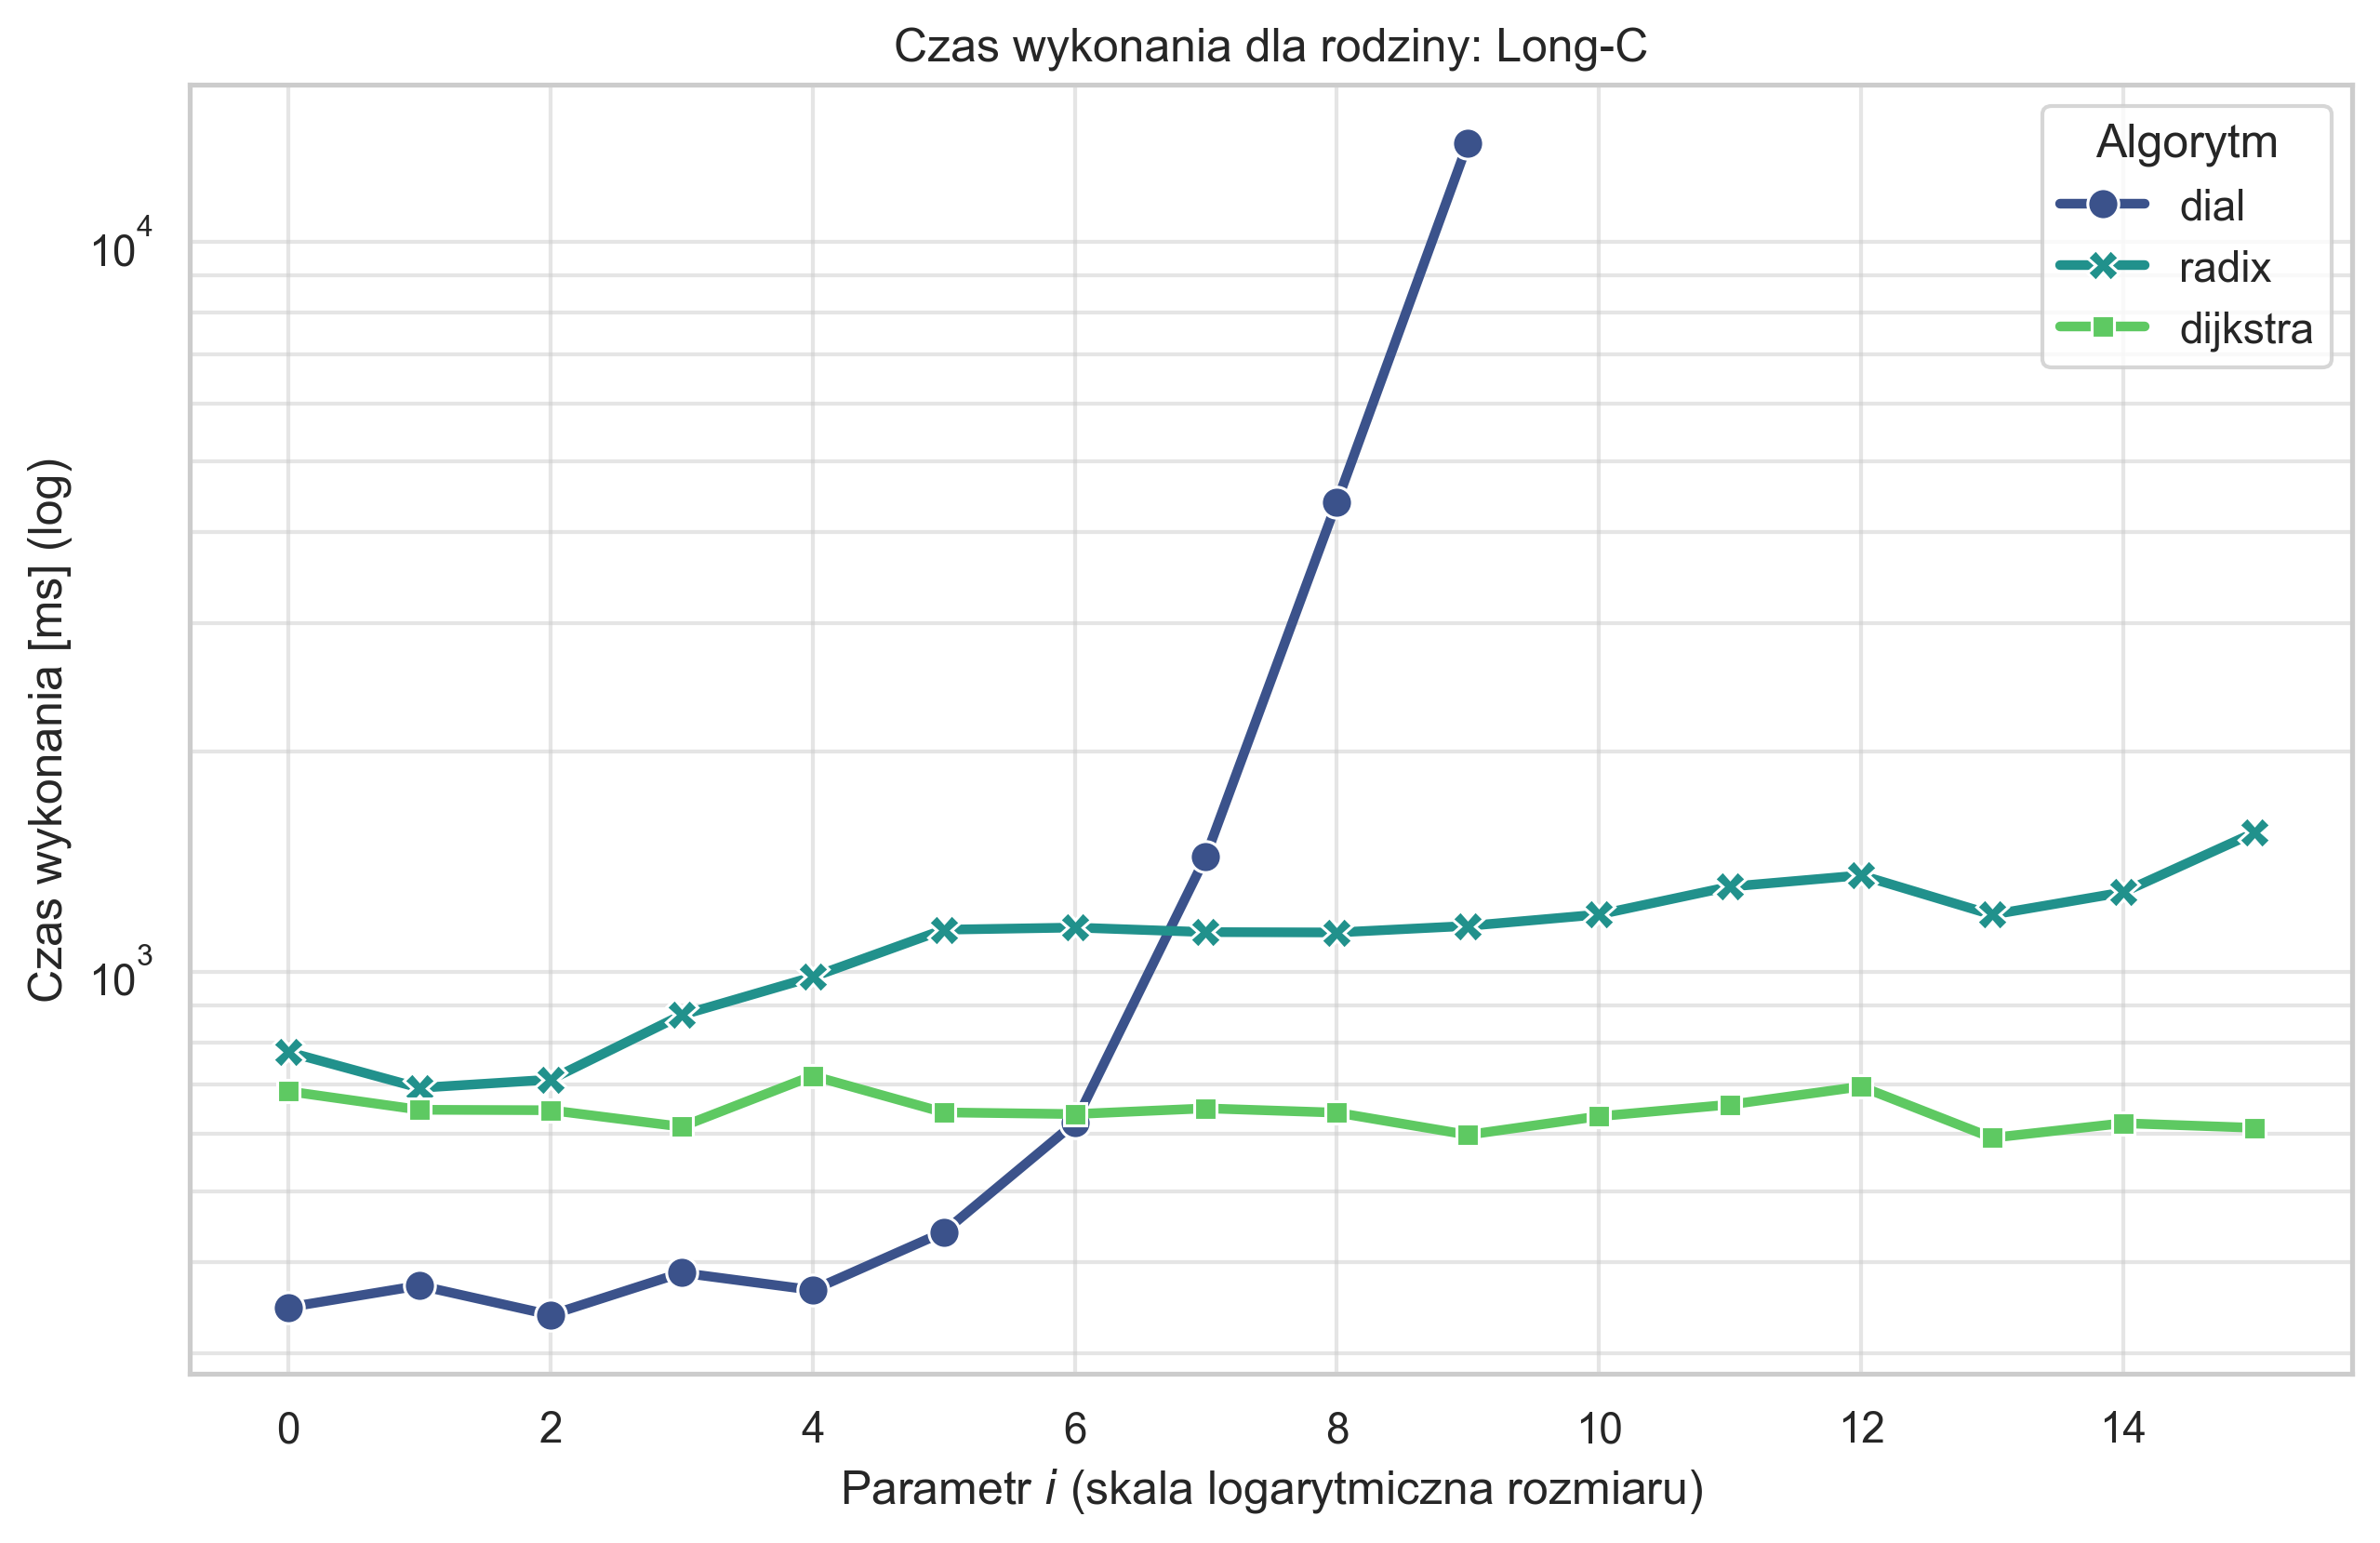
\includegraphics[width=0.9\textwidth]{graphs/random/plot_Long-C.png}
		\caption{Czas wykonywania dla trzech algorytmow (ss5) dla Long-c.}
		\label{fig:longc_random}
	\end{figure}
	
		\begin{figure}[h!]
		\centering
		
\includegraphics[width=0.9\textwidth]{graphs/single/plot_Long-n.png}
		\caption{Czas wykonywania dla trzech algorytmow (ss1) dla Long-n.}
		\label{fig:longn_single}
	\end{figure}
	
	\begin{figure}[h!]
		\centering
		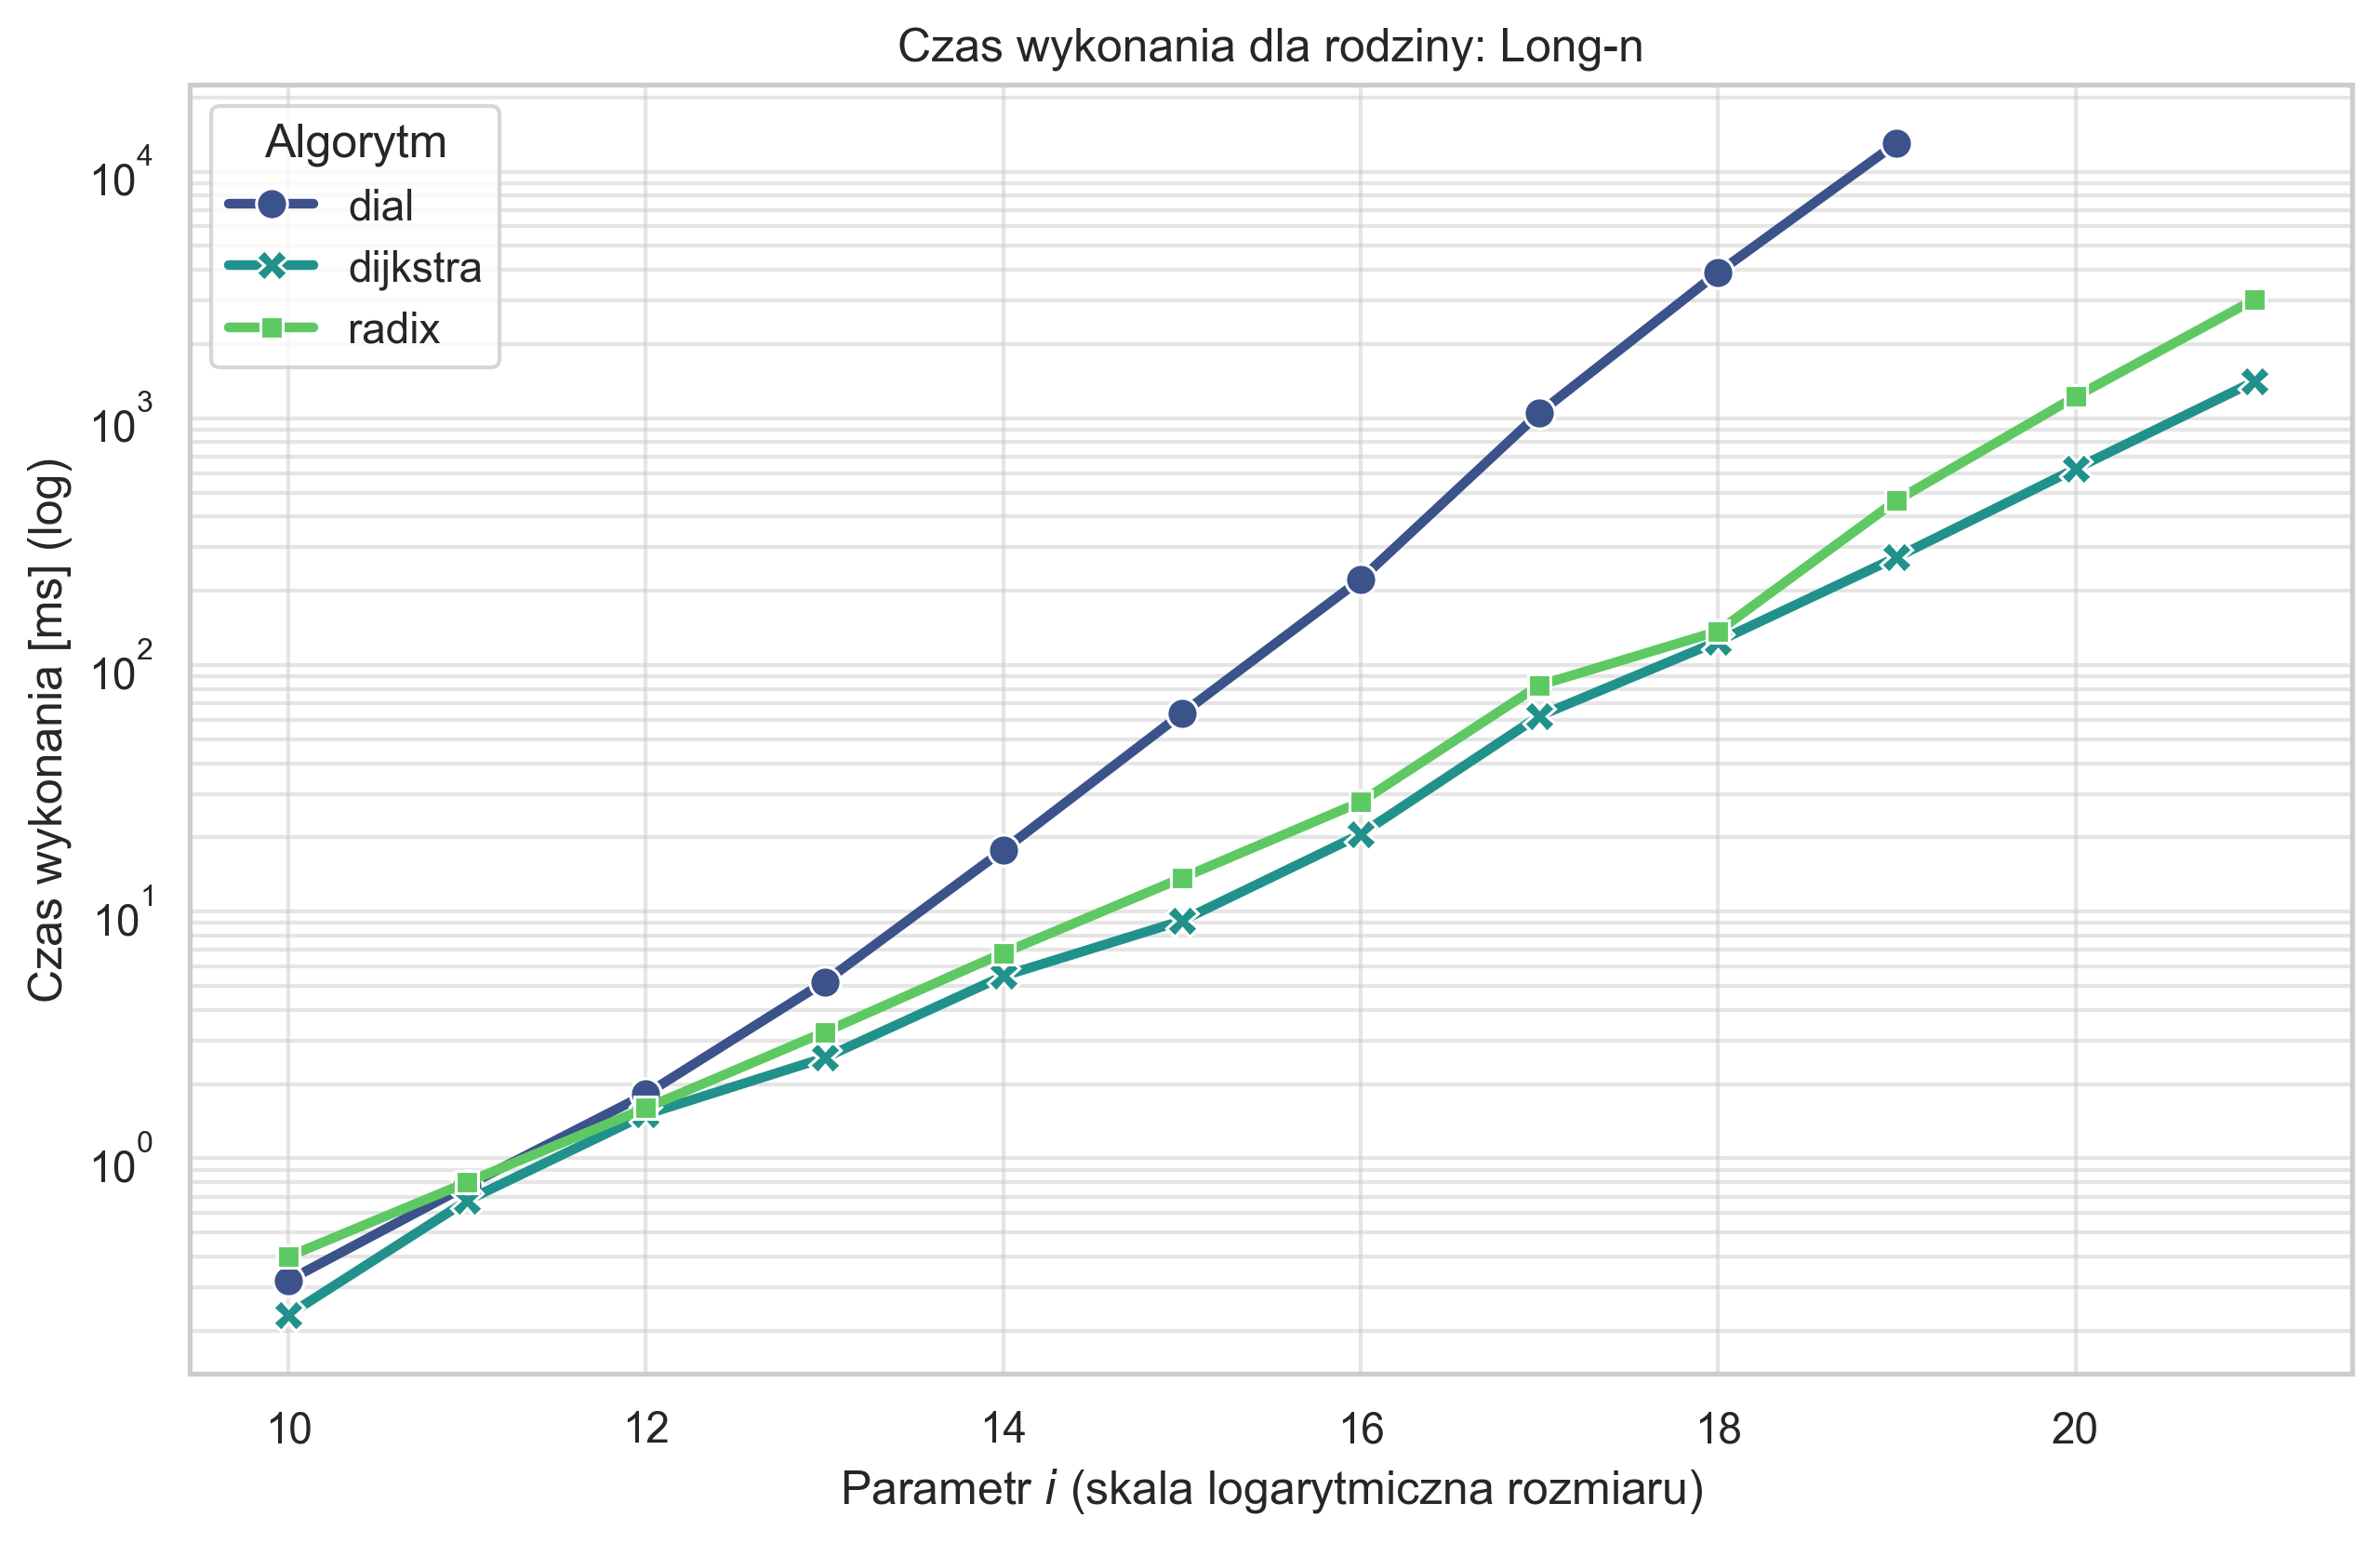
\includegraphics[width=0.9\textwidth]{graphs/random/plot_Long-n.png}
		\caption{Czas wykonywania dla trzech algorytmow (ss5) dla Long-n.}
		\label{fig:longn_random}
	\end{figure}
	
	\begin{figure}[h!]
	\centering
	
\includegraphics[width=0.9\textwidth]{graphs/single/plot_Random4-C.png}
	\caption{Czas wykonywania dla trzech algorytmow (ss1) dla Random4-C.}
	\label{fig:randomc_single}
\end{figure}

\begin{figure}[h!]
	\centering
	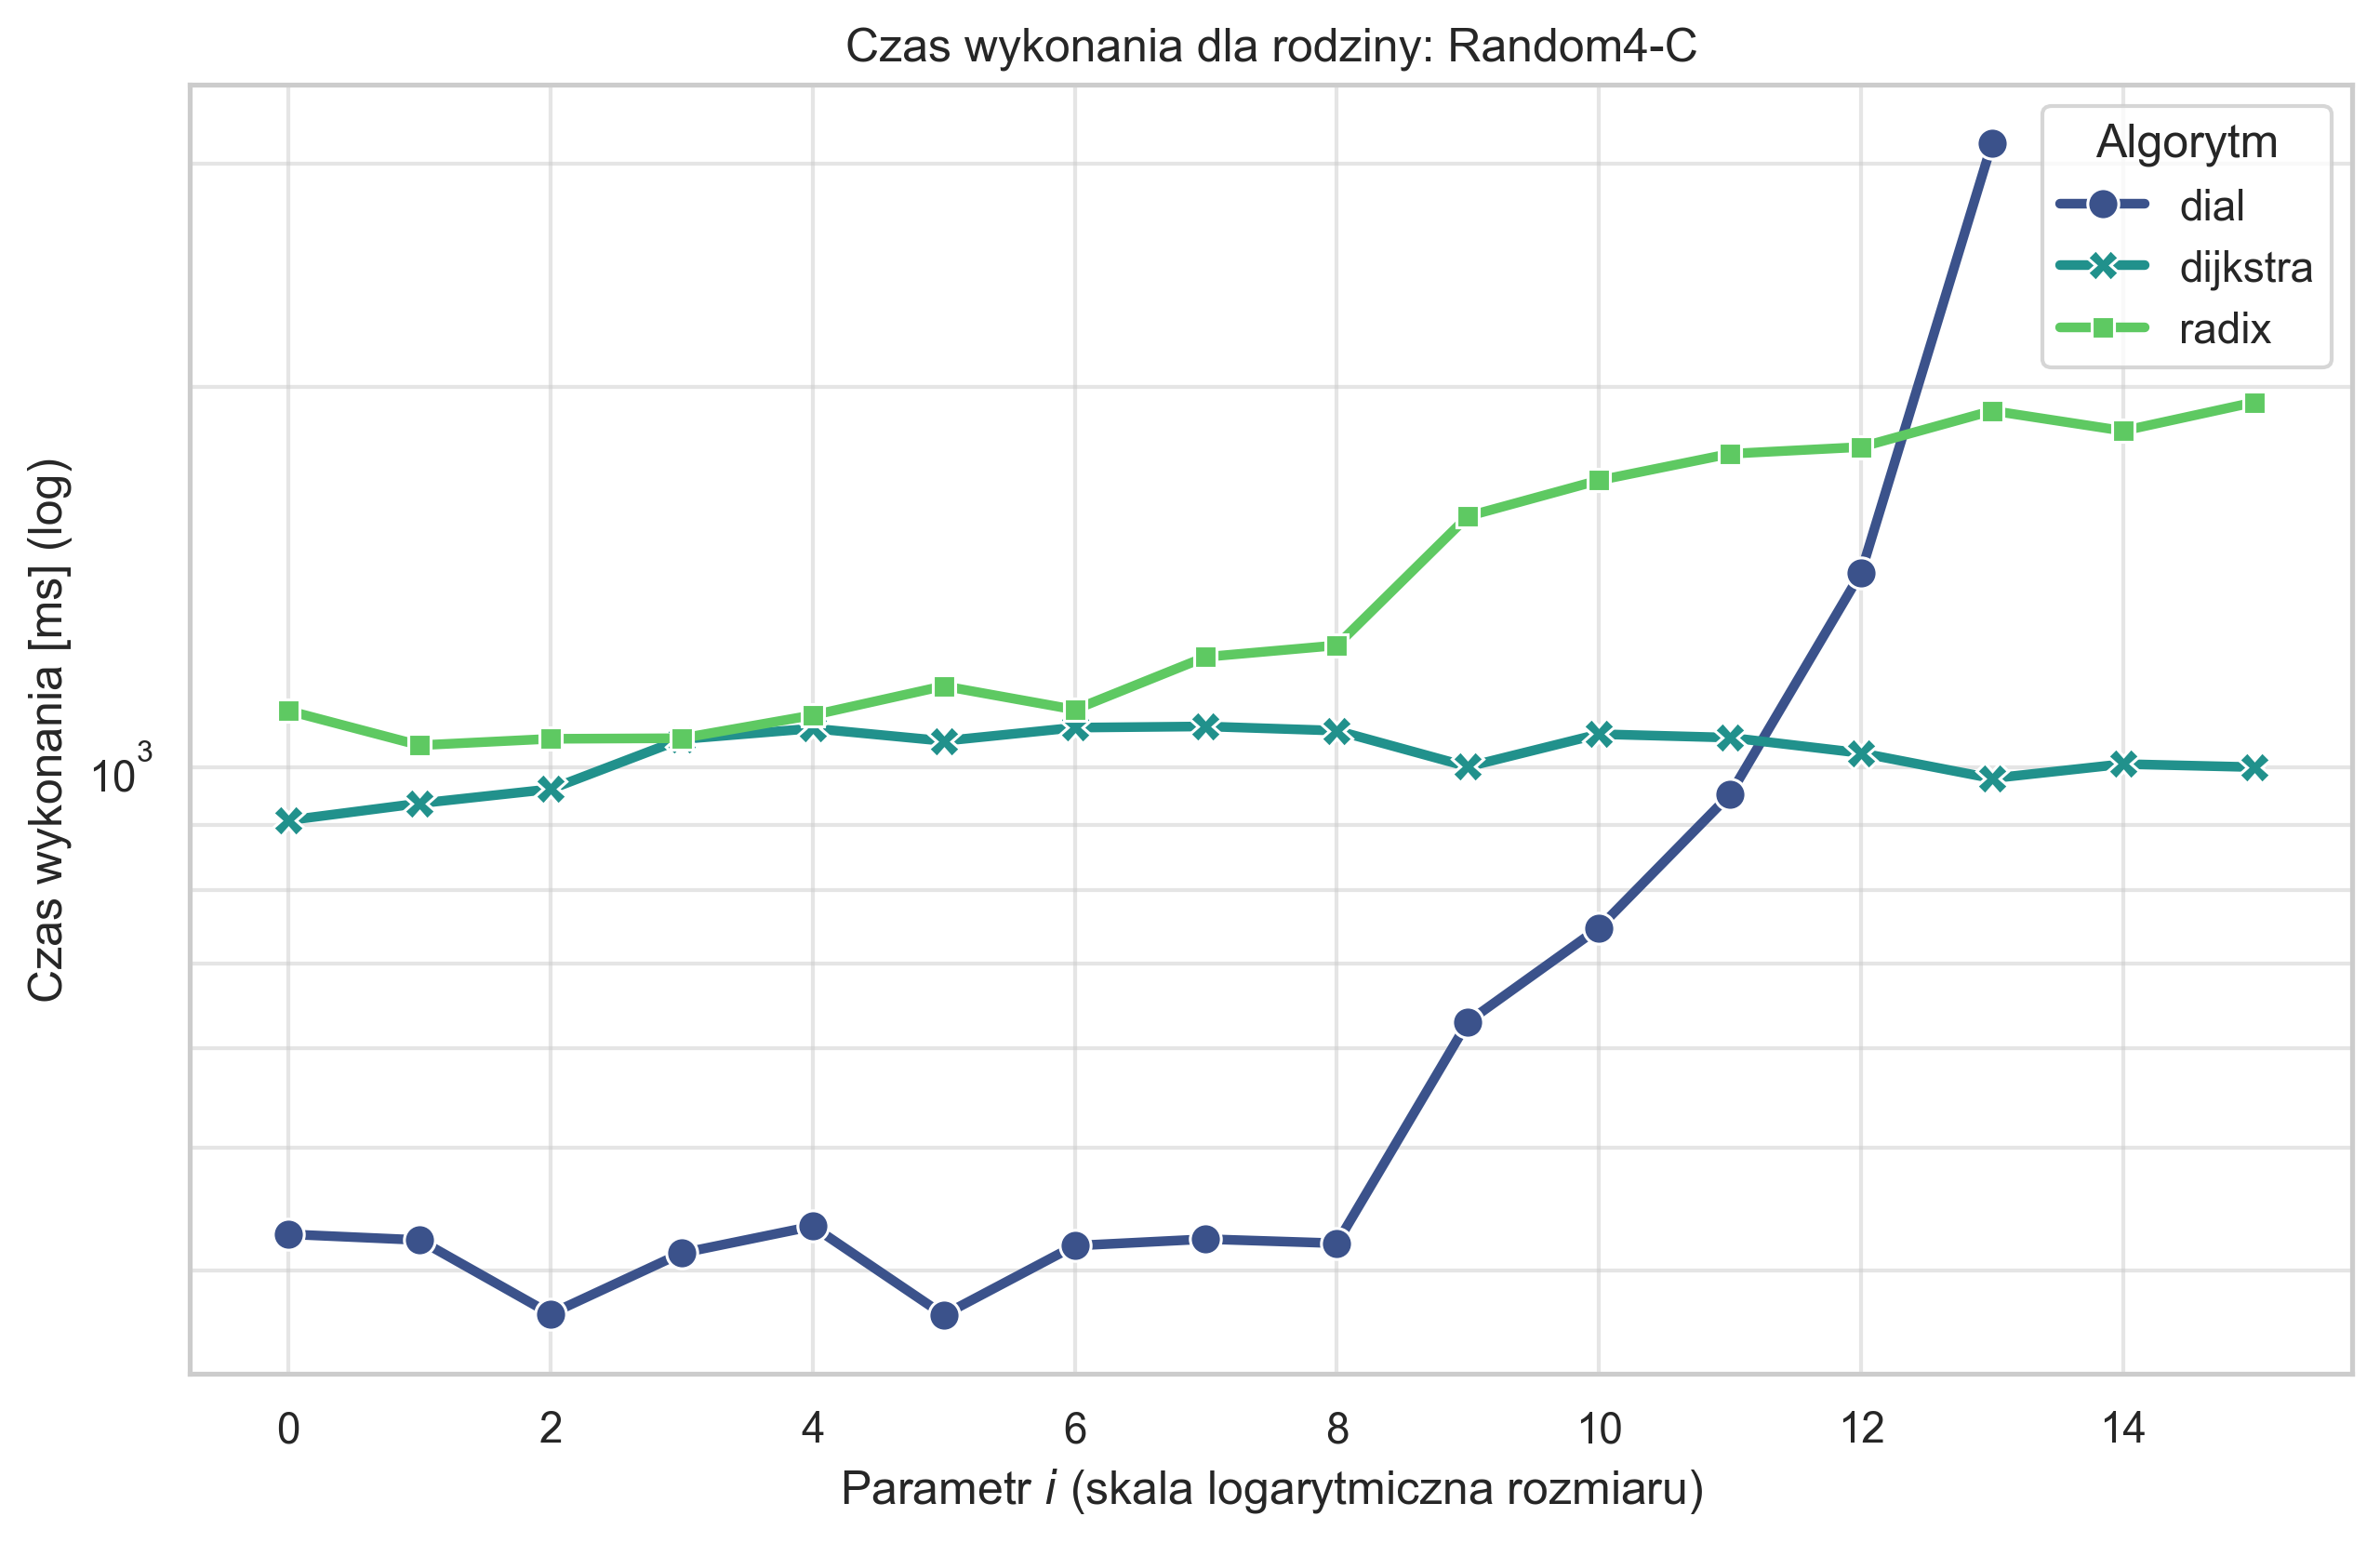
\includegraphics[width=0.9\textwidth]{graphs/random/plot_Random4-C.png}
	\caption{Czas wykonywania dla trzech algorytmow (ss5) dla Random4-C.}
	\label{fig:randomC_random}
\end{figure}

\begin{figure}[h!]
	\centering
	
\includegraphics[width=0.9\textwidth]{graphs/single/plot_Random4-n.png}
	\caption{Czas wykonywania dla trzech algorytmow (ss1) dla Random4-n.}
	\label{fig:randomn_single}
\end{figure}

\begin{figure}[h!]
	\centering
	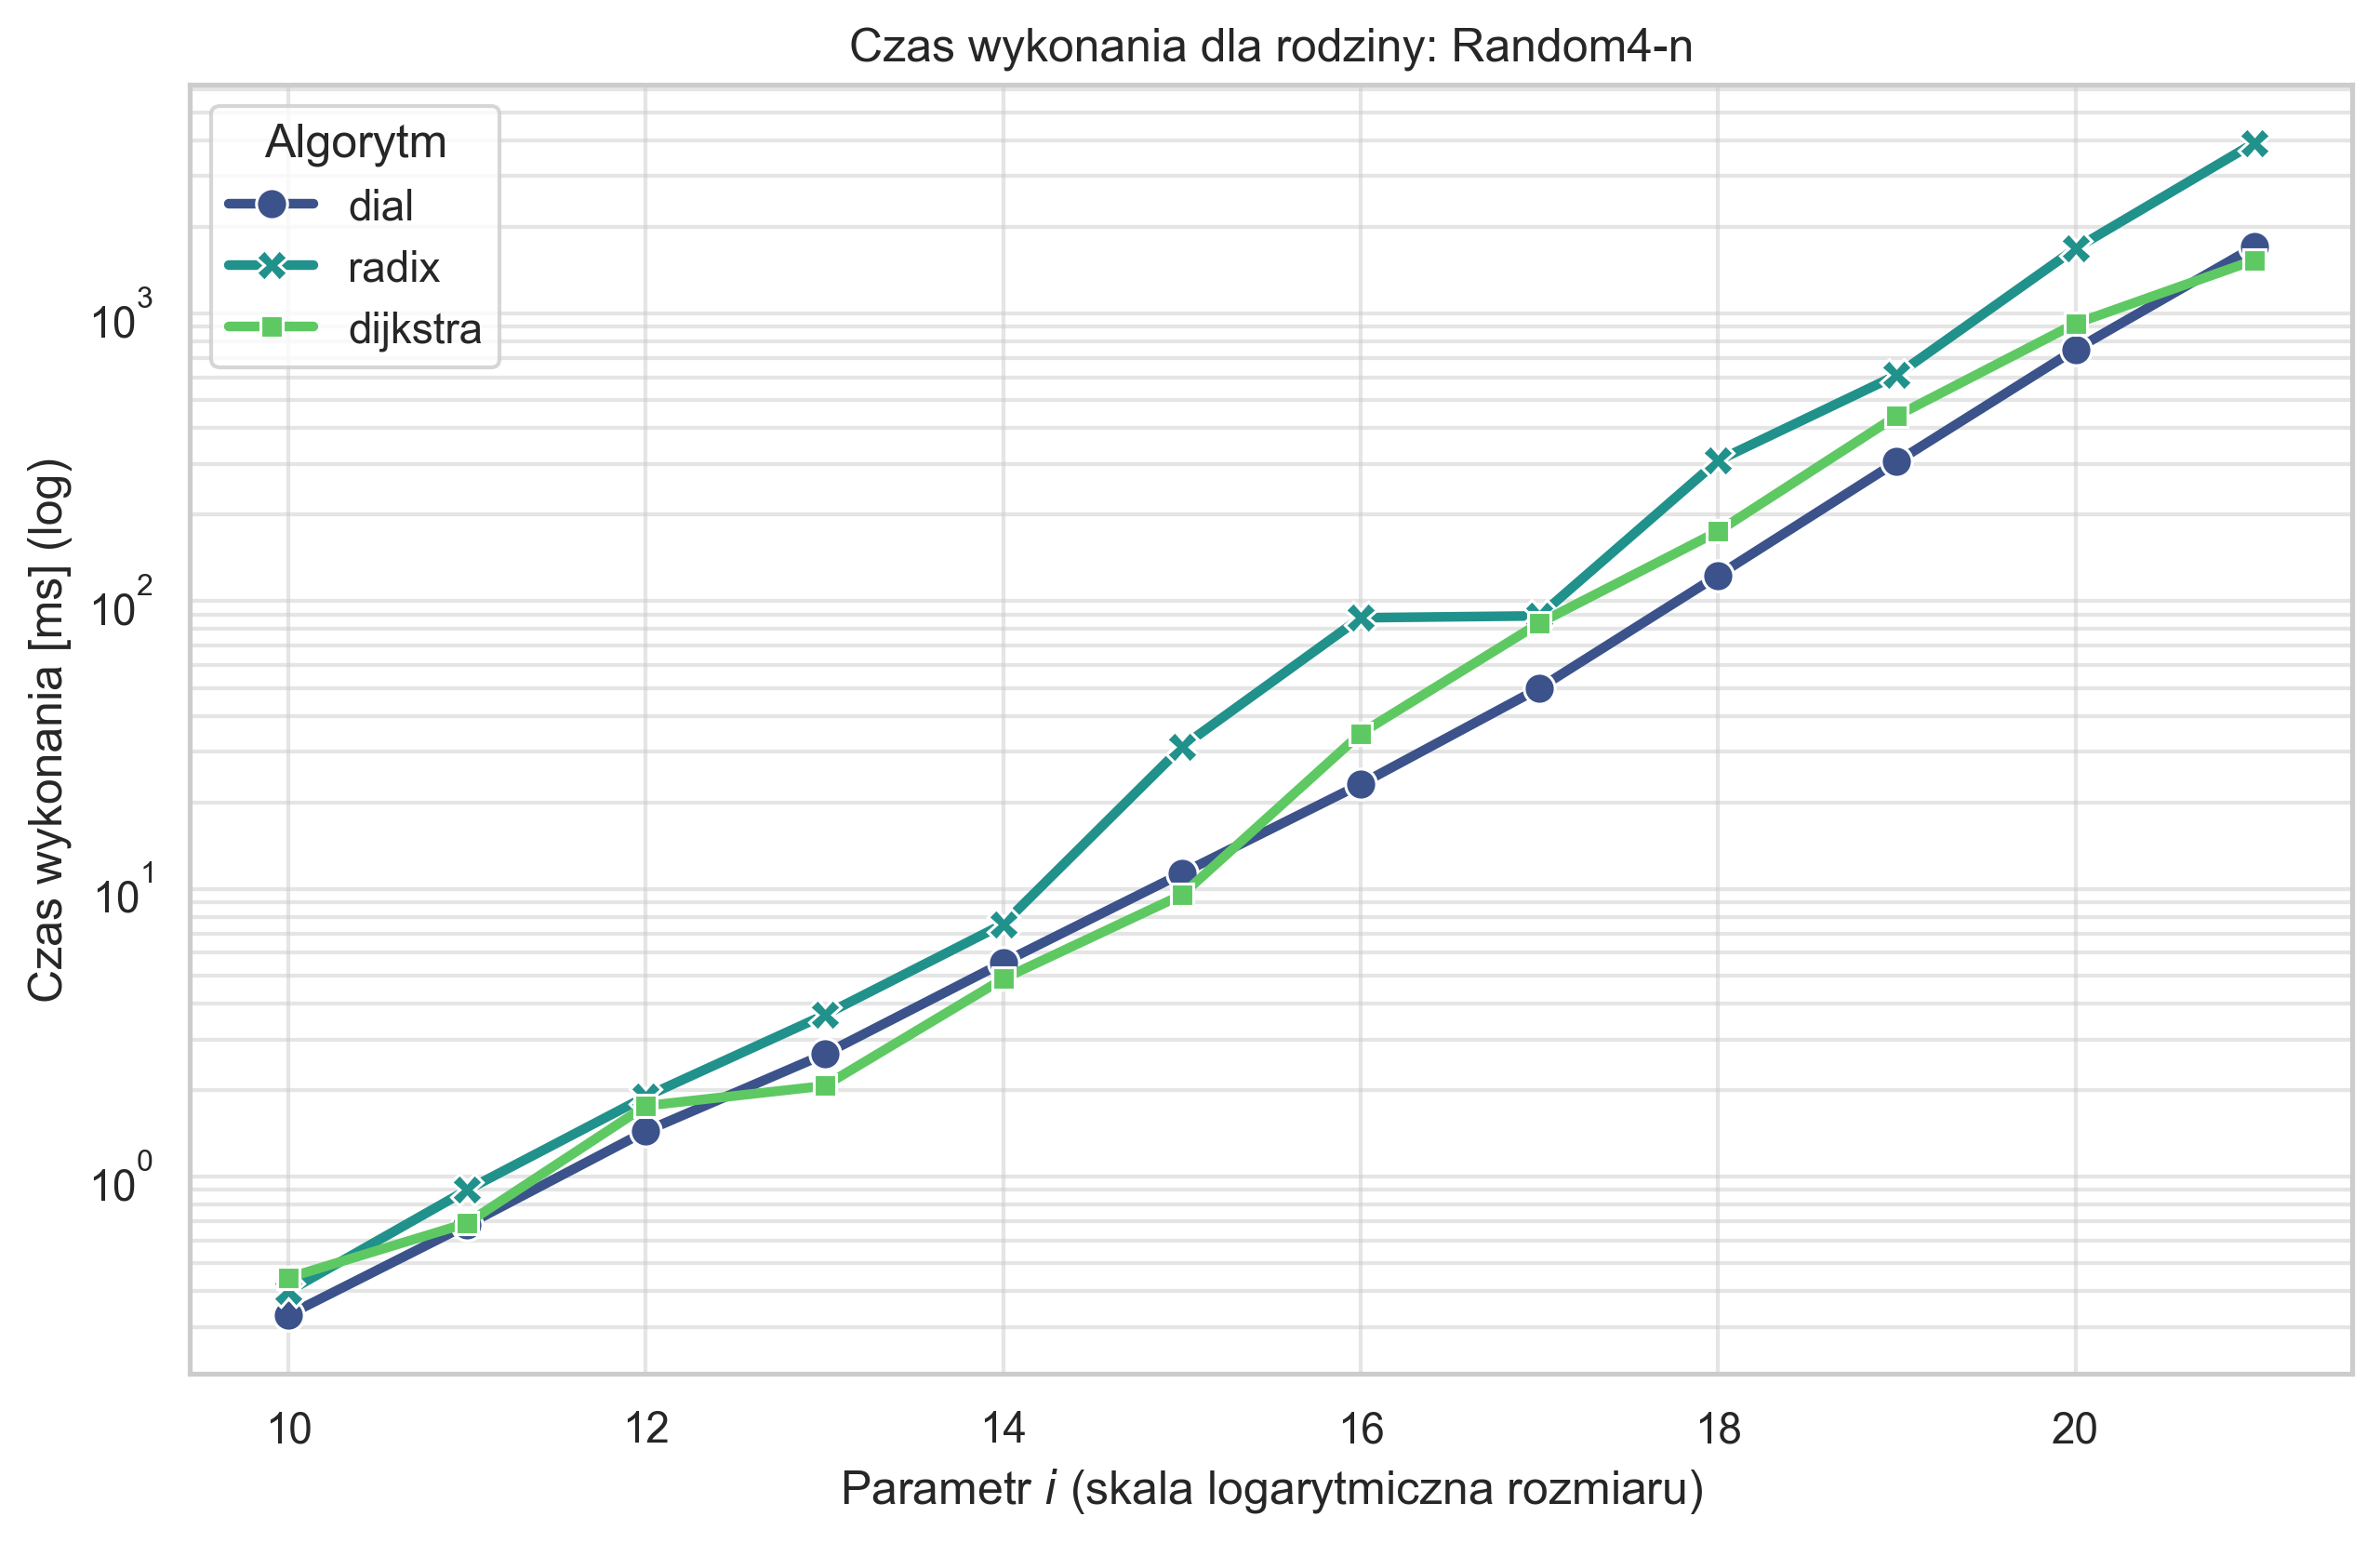
\includegraphics[width=0.9\textwidth]{graphs/random/plot_Random4-n.png}
	\caption{Czas wykonywania dla trzech algorytmow (ss5) dla Random4-n.}
	\label{fig:randomn_random}
\end{figure}

	\begin{figure}[h!]
	\centering
	
\includegraphics[width=0.9\textwidth]{graphs/single/plot_Square-C.png}
	\caption{Czas wykonywania dla trzech algorytmow (ss1) dla Square-c.}
	\label{fig:square_single}
\end{figure}

\begin{figure}[h!]
	\centering
	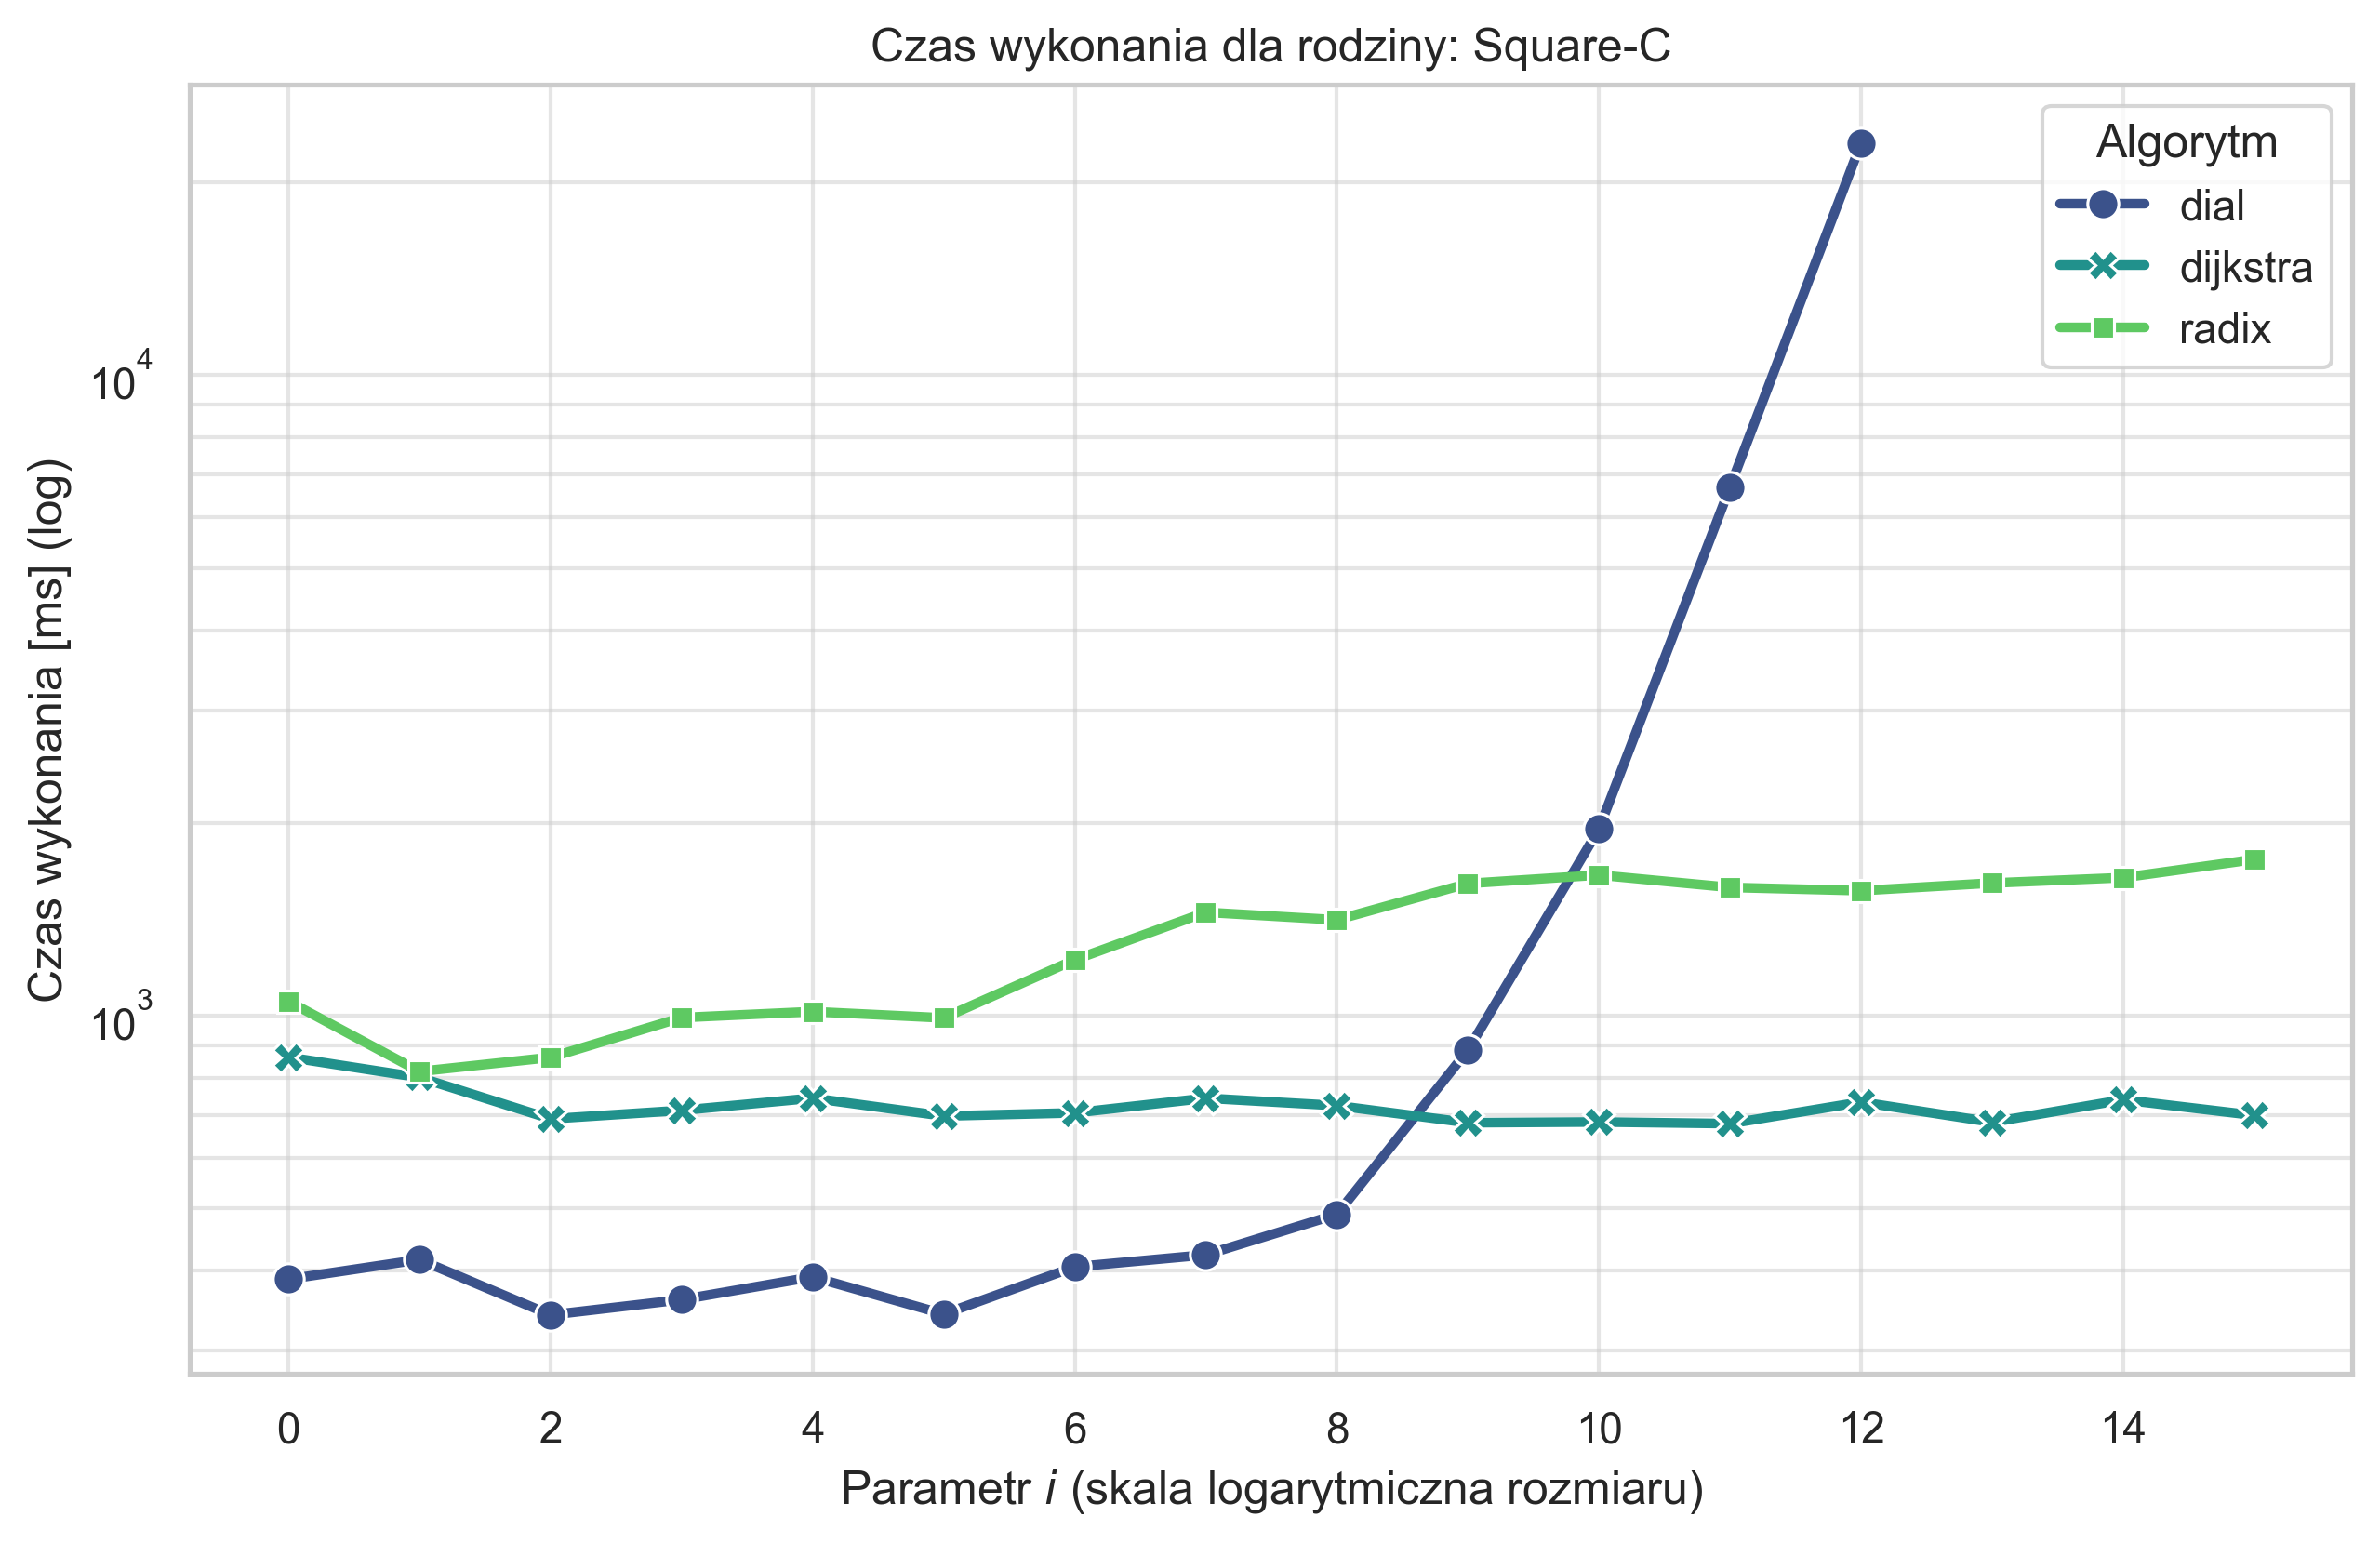
\includegraphics[width=0.9\textwidth]{graphs/random/plot_Square-C.png}
	\caption{Czas wykonywania dla trzech algorytmow (ss5) dla Square-c.}
	\label{fig:lsquarec_random}
\end{figure}

	\begin{figure}[h!]
	\centering
	
\includegraphics[width=0.9\textwidth]{graphs/single/plot_Square-n.png}
	\caption{Czas wykonywania dla trzech algorytmow (ss1) dla Square-n.}
	\label{fig:squaren_single}
\end{figure}

\begin{figure}[h!]
	\centering
	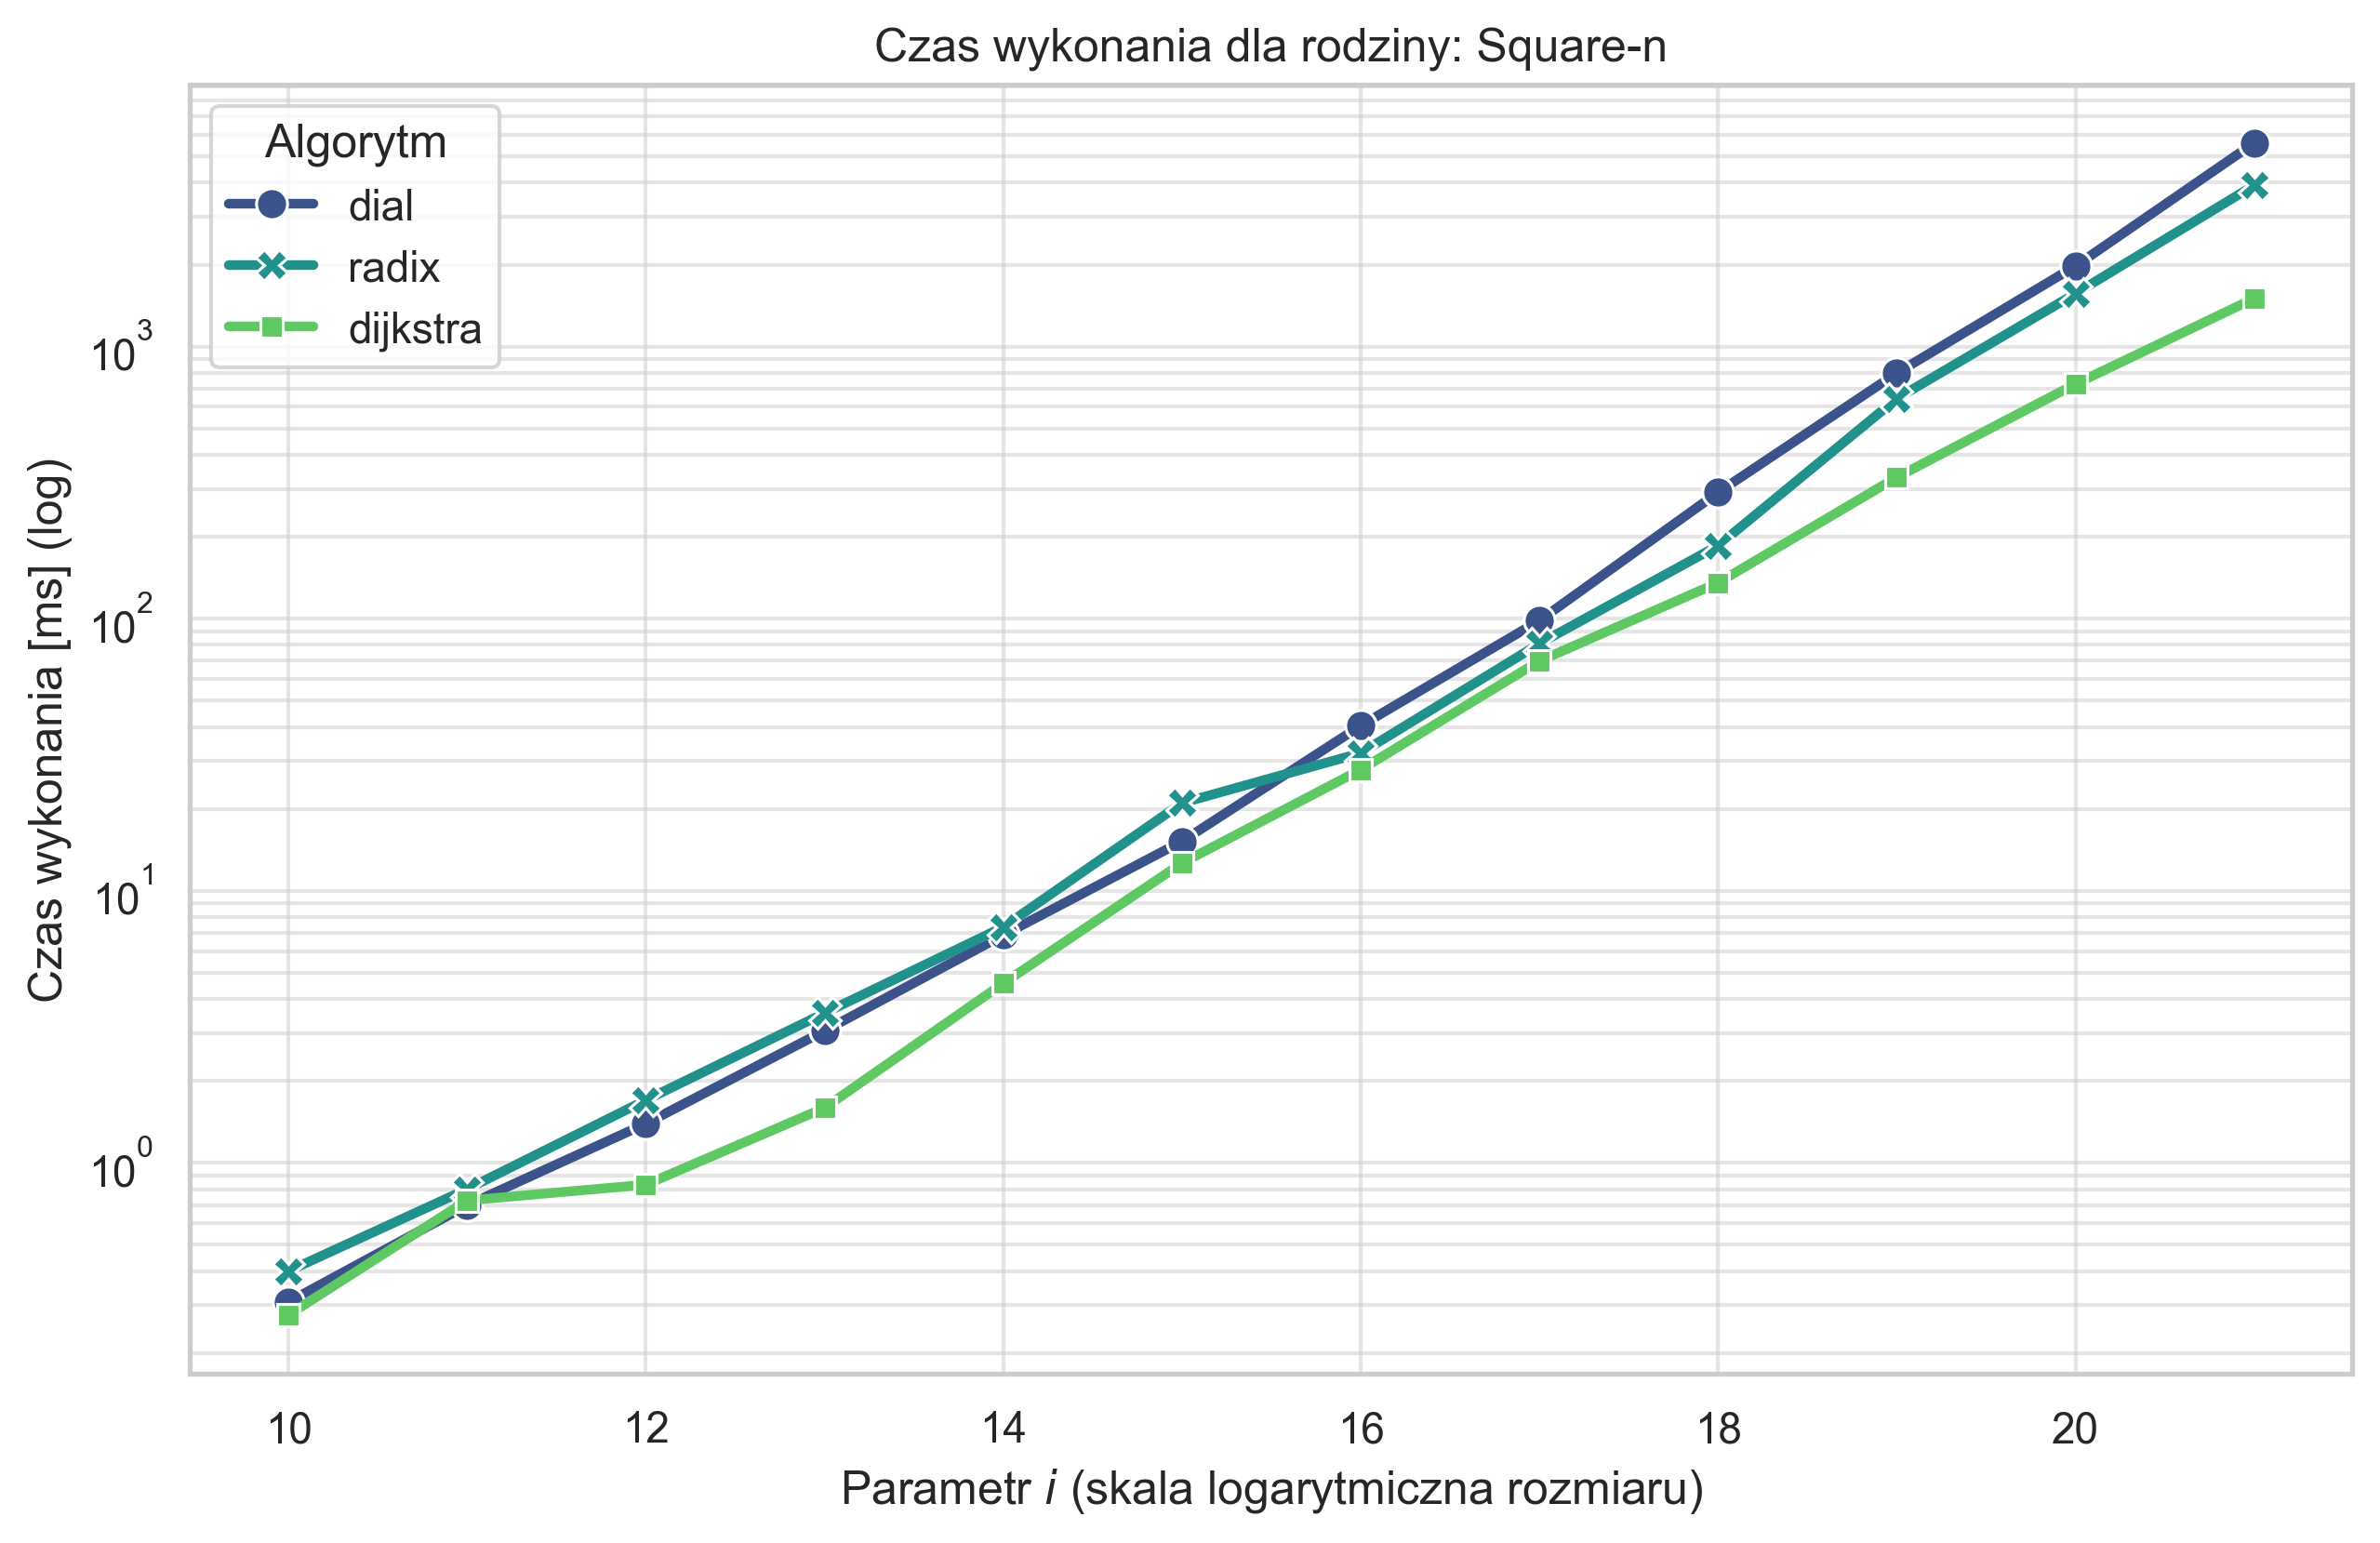
\includegraphics[width=0.9\textwidth]{graphs/random/plot_Square-n.png}
	\caption{Czas wykonywania dla trzech algorytmow (ss5) dla Square-n.}
	\label{fig:squaren_random}
\end{figure}

\begin{figure}[h!]
	\centering
	
\includegraphics[width=0.9\textwidth]{graphs/single/plot_USA-road-d.png}
	\caption{Czas wykonywania dla trzech algorytmow (ss1) dla USA-Road.}
	\label{fig:usa}
\end{figure}

\begin{figure}[h!]
	\centering
	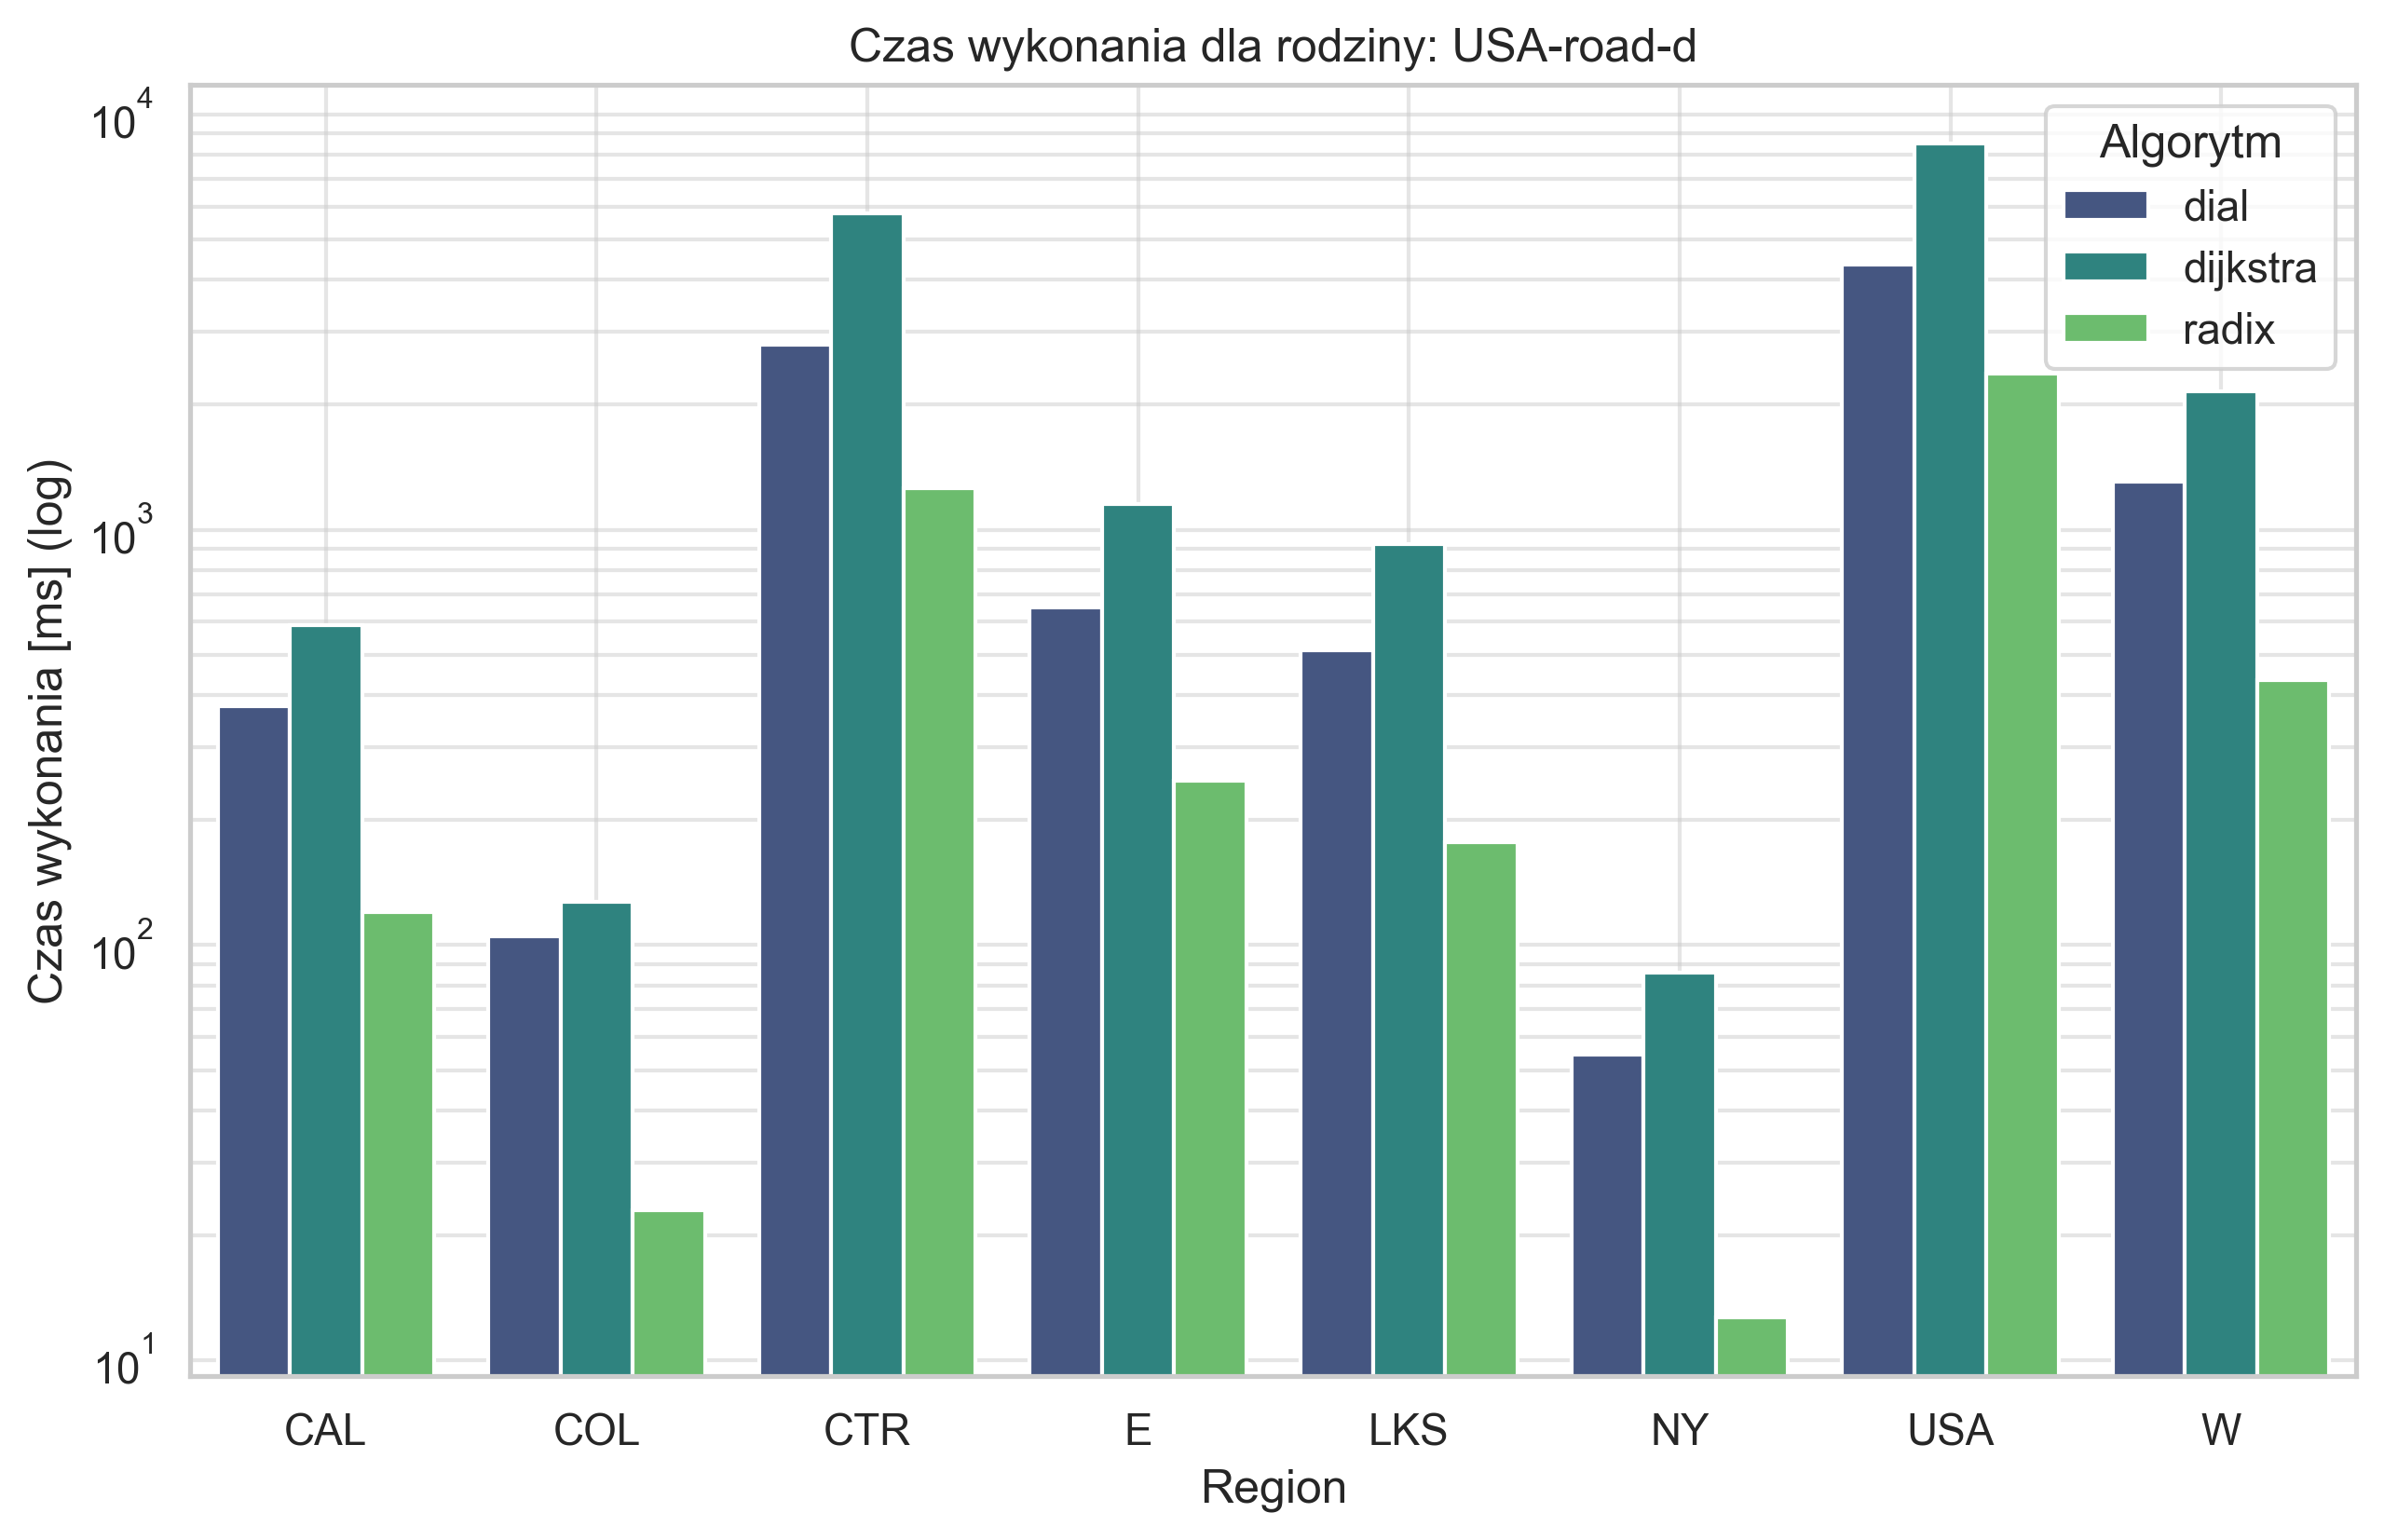
\includegraphics[width=0.9\textwidth]{graphs/random/plot_USA-road-d.png}
	\caption{Czas wykonywania dla trzech algorytmow (ss5) dla USA-Road.}
	\label{fig:usa-random}
\end{figure}
	
	
\section{Wyniki P2P}

\begin{table}[h!]
	\centering
	\caption{Wyniki dystansów P2P}
	\label{tab:radix_p2p_synthetic}
	\vspace{0.2cm}
	\begin{tabular}{lrrr}
		\toprule
		\textbf{Rodzina} & \textbf{Źródło ($s$)} & \textbf{Cel ($t$)} & \textbf{Dystans ($d$)} \\
		\midrule
		\multirow{5}{*}{Long-C} 
		& 1 & 1048576 & 1308259008765 \\
		& 1020739 & 356274 & 2828374846948 \\
		& 992441 & 502136 & 3851590958520 \\
		& 319068 & 830841 & 17660916808358 \\
		& 682655 & 25763 & 2769304432833 \\
		\midrule
		\multirow{5}{*}{Long-n} 
		& 1 & 2097152 & 31336751771 \\
		& 1393665 & 1936822 & 16366943953 \\
		& 621214 & 367017 & 32219787615 \\
		& 583982 & 257908 & 72812309807 \\
		& 1400892 & 1753418 & 53725884992 \\
		\midrule
		\multirow{5}{*}{Random4-C} 
		& 1 & 1048576 & 3471241820 \\
		& 1031144 & 413310 & 4194295948 \\
		& 538881 & 529586 & 4701009828 \\
		& 274254 & 204651 & 4898154363 \\
		& 734648 & 858478 & 4375358684 \\
		\midrule
		\multirow{5}{*}{Random4-n} 
		& 1 & 2097152 & 9051281 \\
		& 1567009 & 643290 & 7979250 \\
		& 15310 & 1447435 & 7656685 \\
		& 673877 & 443339 & 7903017 \\
		& 1724061 & 1881355 & 8682632 \\
		\midrule
		\multirow{5}{*}{Square-C} 
		& 1 & 1048576 & 122219500320 \\
		& 442751 & 411692 & 84374088018 \\
		& 443039 & 921479 & 90471602975 \\
		& 492353 & 82344 & 276379544682 \\
		& 880929 & 434974 & 150123094312 \\
		\midrule
		\multirow{5}{*}{Square-n} 
		& 1 & 2096704 & 714640488 \\
		& 48073 & 926519 & 838476895 \\
		& 2082777 & 583048 & 429845525 \\
		& 333465 & 569378 & 344469271 \\
		& 1289315 & 1676594 & 918089137 \\
		\bottomrule
	\end{tabular}
\end{table}

\begin{table}[h!]
	\centering
	\caption{Wyniki P2P (Mapy USA)}
	\label{tab:usa_radix_p2p}
	\vspace{0.2cm}
	\begin{tabular}{lrrr}
		\toprule
		\textbf{Region} & \textbf{Źródło ($s$)} & \textbf{Cel ($t$)} & \textbf{Dystans ($d$)} \\
		\midrule
		\multirow{5}{*}{BAY} & 1 & 321270 & 2357321 \\
		& 226712 & 47027 & 930499 \\
		& 218825 & 292545 & 1551620 \\
		& 95424 & 236568 & 1212896 \\
		& 53409 & 200873 & 631150 \\
		\midrule
		\multirow{5}{*}{CAL} & 1 & 1890815 & 6570773 \\
		& 459130 & 4852 & 5778572 \\
		& 433536 & 80990 & 6820382 \\
		& 1118467 & 1240065 & 6076316 \\
		& 1287768 & 553527 & 6479109 \\
		\midrule
		\multirow{5}{*}{COL} & 1 & 435666 & 7938506 \\
		& 83973 & 385817 & 6278952 \\
		& 185181 & 338089 & 5892169 \\
		& 65267 & 253938 & 1489374 \\
		& 144095 & 237282 & 2389394 \\
		\midrule
		\multirow{5}{*}{CTR} & 1 & 14081816 & 9709456 \\
		& 4424642 & 6603032 & 6369167 \\
		& 12581034 & 715046 & 25774624 \\
		& 4631693 & 2859817 & 973096 \\
		& 8398368 & 10527027 & 18381750 \\
		\midrule
		\multirow{5}{*}{E} & 1 & 3598623 & 5807795 \\
		& 533051 & 1958286 & 1841074 \\
		& 1659555 & 539859 & 7868941 \\
		& 859101 & 1301000 & 4786996 \\
		& 618475 & 111900 & 3496642 \\
		\midrule
		\multirow{5}{*}{FLA} & 1 & 1070376 & 6371723 \\
		& 11880 & 657561 & 3773721 \\
		& 772549 & 804066 & 917675 \\
		& 754723 & 846660 & 2985092 \\
		& 85419 & 786945 & 4824106 \\
		\midrule
		\multirow{5}{*}{LKS} & 1 & 2758119 & 3051430 \\
		& 2406561 & 811586 & 9758915 \\
		& 1764062 & 173094 & 14118951 \\
		& 1641795 & 924351 & 4057744 \\
		& 121893 & 1689224 & 12981187 \\
		\midrule
		\multirow{5}{*}{NE} & 1 & 1524453 & 2670738 \\
		& 576363 & 1287654 & 3401432 \\
		& 474174 & 1173947 & 4211047 \\
		& 1170710 & 740065 & 4074890 \\
		& 899687 & 565946 & 2181642 \\
		\midrule
		\multirow{5}{*}{NW} & 1 & 1207945 & 8226325 \\
		& 1074483 & 8722 & 10490397 \\
		& 128891 & 853971 & 8423394 \\
		& 553414 & 286016 & 7126692 \\
		& 322086 & 637722 & 5006719 \\
		\midrule
		\bottomrule
	\end{tabular}
\end{table}

\begin{table}[h!]
	\centering
	\caption{Wyniki P2P (Mapy USA)}
	\label{tab:usa_radixs_p2p}
	\vspace{0.2cm}
	\begin{tabular}{lrrr}
		\toprule
		\textbf{Region} & \textbf{Źródło ($s$)} & \textbf{Cel ($t$)} & \textbf{Dystans ($d$)} \\
		\midrule
		\multirow{5}{*}{NY} & 1 & 264346 & 734269 \\
		& 76697 & 365 & 1179607 \\
		& 119470 & 216758 & 1462402 \\
		& 11978 & 174801 & 599276 \\
		& 50836 & 171878 & 773542 \\
		\midrule
		\multirow{5}{*}{W} & 1 & 6262104 & 16307906 \\
		& 2362520 & 581352 & 1248927 \\
		& 1756190 & 1397912 & 3353407 \\
		& 3373116 & 2181780 & 23439897 \\
		& 224495 & 1227050 & 15851432 \\
		\midrule
		\multirow{5}{*}{USA} & 1 & 23947347 & 26227528 \\
		& 2631732 & 21104226 & 25877356 \\
		& 5243200 & 3340168 & 41910239 \\
		& 19359898 & 1926023 & 32457054 \\
		& 16329437 & 21506610 & 19805067 \\
		\midrule
		\bottomrule
	\end{tabular}
\end{table}

\clearpage
\section{Interpretacja wyników i wnioski}

\subsection{Interpretacja wyników}

Uzyskane wyniki eksperymentów dla problemu SSSP wyraźnie odzwierciedlają teoretyczną złożoność czasową każdego z algorytmów.

\begin{enumerate}
	\item \textbf{Algorytm Dijkstry (Kopiec Binarny):} Na wszystkich testowanych rodzinach grafów, wariant z kopcem binarnym wykazał stabilne, ale rzadko najlepsze czasy. Zgodnie ze złożonością $\mathbf{O((n+m) \log n)}$, jego wydajność jest silnie powiązana z liczbą wierzchołków i krawędzi (topologią grafu), lecz pozostaje niezależna od maksymalnej wartości wagi $C$. Na wykresach skalowania (np. dla rodziny \textit{Long-C}), linia Dijkstry jest niemal płaska, co potwierdza odporność na duży zakres wag.
	
	\item \textbf{Algorytm Diala:}
	\begin{itemize}
		\item \textbf{Małe Wagi:} W przypadku grafów o małych wagach (np. $C=1$ w rodzinie \textit{Square} lub \textit{Long-C} dla małego $i$), Dial był bezkonkurencyjny, osiągając wydajność liniową $\mathbf{O(n+m)}$.
		\item \textbf{Duże Wagi:} Dla grafów syntetycznych, gdzie maksymalna waga $C$ rośnie wykładniczo (rodziny oznaczone '-C'), wydajność Diala ulega drastycznej degradacji. Czas wykonania jest wprost proporcjonalny do $C$, zgodnie ze złożonością $\mathbf{O(m + nC)}$, co czyni ten algorytm niepraktycznym przy dużych wartościach wag. Na wykresie skalowania widać gwałtowny wzrost czasu wykonania Diala wraz ze wzrostem $C$.
	\end{itemize}
	
	\item \textbf{Algorytm Radix Heap:} Wariant ten okazał się najbardziej wszechstronny.
	\begin{itemize}
		\item W środowisku małych wag działał niemal tak szybko, jak algorytm Diala.
		\item Dla dużych wag $C$ (tam, gdzie Dial zawodził), Radix Heap utrzymywał niski czas wykonania, porównywalny lub lepszy od standardowej Dijkstry, co jest zgodne ze złożonością $\mathbf{O\left(m + n \cdot \log C\right)}$. Logarytmiczny wzrost względem $C$ czyni go bardzo odpornym na duży zakres wag, co jest kluczowe w praktycznych zastosowaniach.
	\end{itemize}
	
	\item \textbf{Wyniki P2P:} Zgodnie z oczekiwaniami, tabela P2P (\ref{tab:results_p2p_dist}) pokazuje, że wszystkie obliczone dystanse są poprawne (weryfikacja spójności danych), niezależnie od topologii grafu (grafy syntetyczne, sieci drogowe) czy typu zapytania (Min-Max vs. Losowe).
\end{enumerate}

\subsection{Wnioski końcowe}

\begin{itemize}
	\item Wybór optymalnego algorytmu jest zależny od charakterystyki wag:
	\begin{itemize}
		\item Jeśli mamy pewność, że wagi krawędzi są całkowite i małe (np. $C < 1000$), Algorytm Diala jest najlepszym i najszybszym wyborem.
		\item Jeśli wagi krawędzi są duże lub nieznane, a wydajność musi być odporna na duże liczby, Algorytm Radix Heap stanowi optymalne rozwiązanie. Jego wydajność jest logarytmicznie zależna od wag, co zapewnia stabilność i szybkość, czyniąc go faworytem do implementacji w profesjonalnych systemach, zwłaszcza dla danych rzeczywistych (jak \textit{USA-road}), gdzie wagi (np. czas przejazdu) mogą przyjmować bardzo duże, całkowite wartości.
		\item Algorytm Dijkstry (Kopiec Binarny) jest najbardziej uniwersalnym i bezpiecznym wyborem, gdy wagi krawędzi są rzeczywiste lub gdy implementacja struktur danych jest prosta i potrzebujemy gwarancji złożoności niezależnej od $C$.
	\end{itemize}
	
	\item Poprawność: Wszystkie trzy implementacje algorytmów poprawnie wyznaczają najkrótsze ścieżki, co zostało potwierdzone identycznymi wynikami dystansów dla par P2P.
\end{itemize}

	\clearpage
	
\end{document}